\setcounter{chapter}{1} 
\chapter{Theoretical Background} \label{ch:theoretical_back}
Human activity changes the envionments, while the globe need to support the lives of a increasing population. Providing a realistic estimate of future climates is important for motivating mitigation and hopefulle reducing the mean temperature increase. Earth system models, ESM are usefull tool for studing the past and future climate. Observations are used to aid the development of models. It is common to validate a model against observation to ensure that it is capable of describiong the desired mechanisms. 
% Skriv om earth system modells and what their purpose is. Legg vekt på at ting skal være godt nok til å gi et bedre estimat på hva som trengs for å forbedre estimat. (1) cloud or no cloud, (2) Macrophysical properties of clouds such as cloud cover. In NorESM og CESM state of the art earth system models, the joint PDF of humidity, temperature and vertical velocity is used. 
The development of observational system and models requires a understandinng of the physical and biogeochemical processes that takes place in the earth system. Tradeoff between ensuring continous long-term data records and development of retrivals. To include new variables. For capturing the effects of climate change it is beneficial with multidecadal data records. \textbf{Simmons et. al. 2016} The data used in this project is a combination of satellite retrievals and reanalysis data. \textbf{Starting with giving a introduction to clouds in the current and future climate. Continuing with information about the dataset, structure, implementations and practical implications.}

\section{Clouds role in the climate system} \label{sec:cloud_in_climate_system}
% Clouds, climate and machine learning
Clouds play an important role in the climate system both affecting the radiative budget and the hydrological cycle. Understanding how clouds form in the complex system of the atmosphere involves both knowledge about the large scale influence by the circulation and the small scale influence by aerosols. Clouds exist in countless number of shapes and sizes, and have fascinated mankind since the beginning of time. Figure \ref{fig:cloud_cover_jotunheimen} shows the stunning view from Store Smørstabbtinden in Jotunheimen. The sky is covered by cumulus type clouds, a common sight in summer.
\begin{figure}
    \centering
    \adjincludegraphics[scale=0.1, trim={0 {.3\height} 0 0}, clip]{Chapter1_Intro/images/cloud_cover_ina.jpg}
    \caption[Cumulus deck at Store Smørstabbtinden in Jotunheimen]{Cumulus deck at Store Smørstabbtinden in Jotunheimen, photo by Ina Storteig.}
    \label{fig:cloud_cover_jotunheimen}
\end{figure}
%Climate models are the most useful tool for studying the past, present and future climate. Clouds and aerosols are acknowledged as the factors contributing with the largest uncertainty to the \acrfull{ecs}. Also known as global mean temperature increase as a consequence of doubling of the pre-industrial levels of $CO_2$ (280 \acrshort{ppm}). \textbf{kilde AR4 which ch?} \textit{It remains unclear to which level of sophistication is adequate to model their effect om climate.} (\cite{IPCC_CH7_clouds}).
%\newpage

\subsection{Evolution of clouds}
Clouds are composed of liquid droplets, ice crystal or both. To this day the microphysics of all phases are not fully understood \textcolor{red}{\textbf{kilde - les å sjekk at den kan brukes} \cite{ReviewMicroPhys}}. Here mixed phase clouds, consisting of both liquid and ice, have proven to be the most difficult to fully understand. 

\textit{Aerosols} include both liquid and solid particles suspended in the air. They interact with the clouds by serving as particles which vapour and ice can condensate or deposit upon. The different phases require different properties and the nuclei are called \acrfull{ccn} for liquid droplets and \acrfull{inp} for ice crystals. 
% Chemistry definition of saturation - the degree or extent to which something is dissolved or absorbed compared with the maximum possible, usually expressed as a percentage.
In the following discussion, \textit{saturation} describes the equilibrium state between to phases. % \textcolor{red}{er dette en definisjon du selv har funnet på? Eller har det fra et sted? }. 
For phases such as liquid water and vapour, saturation implies equal rates of condensation and evaporation. Phase changes occur when the system deviates from the equilibrium state. Under supersaturated conditions, the rate of condensation exceeds the rate of evaporation, facilitating vapour to condense onto suitable aerosols and initiating the formation of clouds. 
% The energy barrier needed to overcome (surface tension) to homogeneous nucleation 

Saturation is usually achieved by a temperature decrease in rising air masses. The saturation vapour pressure, $e_s$, is the quantity describing the maximum amount of vapour air can retain at a certain temperature. The way in which $e_s$ depends on the temperature, $T$, is described by the Clausius-Clapeyron equation for water, see Equation \eqref{eq:clausius_clapeyron_differentias}. The entalphy of vaporization, $l_v$, is the amount of energy needed to evaporate one unit (e.g one mole) of molecules from the liquid. This is also known as the latent heat of vaporization. 
\begin{equation} \label{eq:clausius_clapeyron_differentias}
    \frac{de_s}{dT} = \frac{l_v e_s}{R T^2}
\end{equation}
Here $l_v = 40.8 \cdot 10^3 J mol^{-1}$ and the universal gas constant $R= 8.314 J mol^{-1} K^{-1}$ (\cite{cloud_phys_book_johanne}, p. 42). 

A solution to Equation \eqref{eq:clausius_clapeyron_differentias} is given in Equation \eqref{eq:clausius_clapeyron}. It is derived by integrating from $T_0 = 273.15K \left(0 ^{\circ}C \right)$ to an arbitrary temperature, $T$. The integral is intractable for varying $l_v$. However a constant $l_v$ is %in most cases 
a reasonable assumption for the ranges of temperatures of atmospheric interest. The lower boundary, $T_0$, is chosen based on convenience, motivated by the fact that the constant of integration,  $e_0$, needs to originate from measurements. At $T_0$, the equilibrium of a mixture of water and ice at a total pressure of $1$ $atm$ is $e_0 = 611Pa$. 
\begin{equation} \label{eq:clausius_clapeyron}
    e_s\left( T \right) = e_0 e^{\frac{l_v}{R} \left( \frac{1}{T_0} - \frac{1}{T} \right) }
\end{equation}
From Equation \eqref{eq:clausius_clapeyron} it is clear that $e_s$ increases with rising temperature, resulting in the phenomena that warmer air can retain more vapour. The same principles apply for the phase change sublimation, but its entalphy, $l_s$, has a distinct value (\cite{cloud_phys_book_johanne}, p.135). The saturation vapour pressure with respect to ice, $e_i$, can be derived by replacing $l_v$ by $l_s$. Subsaturated conditions cause the cloud liquid water to evaporate, and ultimately the cloud disappears. This can happen when the cloud mixes with dry air or the temperature increase. The reverse process of adiabatic cooling, caused by sinking air masses in cloud. 

%From Equation \eqref{eq:clausius_clapeyron} it becomes clear that the  is inversely proportional with the second power of the temperature, meaning that for decreasing temperatures the vapour pressure 
%Double check if this id only valid for adiabatic processes, is there any other assumptions..?
%$R^*$ is the specific gas constant (the universal
%gas constant divided by the mean atmospheric molecular
%weight).  
Growth processes are phase dependent. Liquid droplets grow by diffusion and later by collision and coalescence. At temperatures around -38 $^oC$ (\cite{lohmann2016}, \textbf{p.222}, men det referes til pruppacher og klett 1997) droplets spontaneously freeze, while at warmer temperatures freezing can only occur with the aid of an  \acrshort{inp}. Clouds consisting purely of ice crystals first grow by deposition of vapour and then by aggregation (\cite{Fowler1996LiquidAssumptions}). In the presence of both phases, the Wegeron-Bergeron-Findeisen process describes the mechanism where droplets evaporate and the vapour deposits on to the ice crystals. %When both phases are present in a cloud, the saturation vapour pressure over ice is higher than over liquid. This may cause the droplets to evaporate and deposit on to the ice crystals. 
This mechanism exists because the saturation vapour pressure is lower with respect to ice than water, $e_i < e_s$. The process is most efficient at -12$^{\circ}C$ when the difference is largest.

%\section{Clouds role in the energy budget}

\subsection{Clouds role in the radiative budget}
\textbf{MOVE TO THE MOST SUITABLE SPOT. Macrophysical properties describe the clouds as units, using properties like base height, top height, thickness, fractional cover and regime (also known as type). Microphysical processes are all mechanisms involving the particles forming a cloud. Examples of properties used to quantify the microphysical state
are \acrshort{ccn} and droplet number concentrations (\cite{Grabowski2019ModelingBetter}).}
The characteristic white colour of the clouds has it nature in its ability to  effectively scatter solar radiation. %(explains why they appear white - because the backscatter radiation of all wavelenght in the visible spectrum)
%In part, this mechanism describes the important role in the Earth radiative budget. 
The Earth bathes in radiation from the Sun. Passing through the atmosphere, a small portion of the radiation gets absorbed while another portion gets scattered by clouds and aerosols. The majority of the radiation reaches the Earth and transforms into heat, warming the surface. The Earth emits thermal radiation, a minor portion of which escapes directly back to space, while most of it gets absorbed by the atmosphere and is re-emitted. This phenomena is known as \textit{the greenhouse effect}. 

The amount of heat trapped in the Earth system depends fundamentally on the spectral properties of its components (i.e. clouds, greenhouse gases, aerosols), and determines the magnitude of the enhanced warming (\cite{greenhouse_effect}).

%The physical properties of the atmospheric components determine their interactions with radiation. 
\textit{Albedo} is the ratio of reflected to incoming radiation. Dense low level clouds have high number concentrations of droplet, which corresponds to a large surface area. This results in enhanced scattering of radiation and thus a higher albedo. The greenhouse effect of clouds follows the principals of the greenhouse effect described above. It arises from their ability to absorb thermal radiation and re-emit it. The absorbed radiation originates from the surface or the atmosphere below. A widely used assumption is that the Earth (and most clouds) radiate like a black body, thus its radiant flux is given by Stefan-Boltzmann fourth-power law, 
\begin{equation} \label{eq:stefan-boltzmann}
    F = \sigma T ^4 % \epsilon
\end{equation}
here $F$ denotes flux in units of $W m^{-2}$, $T$ denotes temperature in units of $K$ and \\  $\sigma = 5.670 \time 10^{-8} W m^{-2} K^{-4}$ is the Stefan-Boltzmann constant. 
%The \textit{emissivity}, $\epsilon$, of a medium is the ratio between the actual emission and the black body emission at the same temperature. It depends on the beams frequency and the viewing angle.
 %Most models assume a black body emission of the Earth and the atmospheric components, this corresponds to an emissivity, $\epsilon=1$. 
%TS: Her ville jeg ikke sagt at modeller antar en emissivitet på 1 for alle "atmospheric components" for det er ikke riktig. For drivhusgassene varierer emissiviteten for ulike diskrete bølgelengde-bånd, men det er jo riktig at disse beregningene er forenklinger og dermed bidrar med usikkerhet


Mediums like water, snow and ice are not necessarily perfect emitters, this requires the need for modifying Equation \eqref{eq:stefan-boltzmann} with a scaling factor, called emissivity, $\epsilon \in [0, 1]$,
%TS: Du har jo allerede introdusert epsilon ovenfor, så litt rart å gjøre det igjen her
this depends on the composition and density of the medium. The emitted flux is given by $ F = \sigma \epsilon T ^4$. This provides an additional source of uncertainty to the computations of the greenhouse effect of clouds and therefore also the \acrshort{ecs}.

%To asses the validity of the black body assumption on the Earth surface, \citepaper{Huang2018ImprovedClimate} demonstrated the changes in the radiative transfer calculations by varying the emissivity based on surface types. Their findings show that it makes a considerable change to the radiative transfer calculations, and in conclusion it need to be further investigated. 
%TS: Teksten ovenfor tar forsåvidt opp et interessant tema, men det er ikke veldig relevant for denne oppgaven...
Researchers are still struggling with determining the exact spectral emissivity of different mediums. This is of interest for both implications to the radiative transfer calculation, but it is also of utmost importance in the field of remote sensing, where distinguishing the signal from the reference signal continues to pose as a problem.
%this property is also being exploited in remote sensing. In remote sensing it is of utmost importance to distinguish the signal from the reference signal, a cloud from its background for instance. 
%Different parts of the globe are covered by different surfaces and \citeauthor{Huang2016AnSimulations} proved that assuming a constant surface emissivity effects the \acrfull{toa} polar energy budget \textbf{read paper again to determine why this is of importance}. 
The greenhouse effect increases with the cloud altitude, enhanced by the increased temperature difference between the surface and cloud. High clouds with low temperatures re-emit radiation at a lower intensity than they absorbed. Energy thereby gets trapped in the Earth system, which has a warming effect. 
%Despite the uncertainties related to emissivity of the medium, the re-emitted radiation is of a lower intensity than what it absorb.
%This is shown in equations \eqref{eq:cre_sw} and \eqref{eq:cre_lw}. \textbf{drop equations..?}
\section{Clouds in the current climate} \label{sec:intro_cloud_current_climate}
On the basis of simulations and available observational data, both remote sensing and in-situ measurements, \citepaper{Wild2019TheModels} have quantified the contribution of elements in the Earth's annual global mean energy budget. The Cloud radiative effect (\acrshort{cre}) is computed by subtracting the components of a cloudy atmosphere from a cloud-free atmosphere (\cite{RAMANATHAN1989}), usually at the top-of-the-atmosphere (\acrshort{toa}). The altitude along with the composition of clouds determine their optical properties and in turn their interactions with radiation.

\begin{figure}[ht]
    \centering
    \definecolor{mygray}{gray}{0.8}

    \begin{tikzpicture} %[remember picture,overlay]
        \node at (current page.center) {\includegraphics[scale = 0.55]{Chapter2_Theory/images/cre_ny_farge.pdf}};
        \begin{scope}
            % Grid to help find the positions (remove in final version)
            \node at (11cm, 19.5cm) {\Large \textcolor{mygray}{Cloud Radiative Effect (CRE)}};
            
            \node at (14.2cm, 18.1cm) {\Large \textcolor{orange}{LW CRE = +28}};
            %\node at (14.7cm, 16cm) {\large 28};
            
            \node at (9cm, 18.1cm) {\Large \textcolor{yellow}{SW CRE = -47}};
            %\node at (8.7cm, 16cm) {\large -47};
            
            
            % Litt usikker på om jeg syns de bidro
            %\node at (16.5cm, 15.4cm) {\large Atmosphere};
            %\node at (17cm, 18cm) {\large TOA};
            %\node at (16.4cm, 10.2cm) {\large Surface};
            
            \node [rotate = 70] at (10.5cm, 11.6cm) {\small \textcolor{red}{sensible heat}};
            \node [rotate = 73] at (9.7cm, 11.7cm) {\small \textcolor{mygray}{latent heat}};
            \node [rotate = 73] at (8.9cm, 11.5cm) {\small \textcolor{mygray}{solar reflected surface}};
            
            \node at (6.1cm, 10.7cm) {\small Imbalance};
            
            \node at (15.9cm, 11.2cm) {\Large 28};
            \node at (15.4cm, 14.1cm) {\Large 0};
            \node at (7.cm, 14.2cm) {\Large 7};
            \node at (11.2cm, 13.2cm) {\Large 7};
            
            \node at (11.3cm, 15.4cm) {\Large NET CRE};
            \node at (11.3cm, 14.9cm) {\Large =-19};
            
            \node at (11.cm, 10.6cm) {\Large -26};
             
            \node at (16.cm, 10.4cm) {\small thermal};
            \node at (16.cm, 10.1cm) {\small down};
            \node at (16.cm, 9.8cm) {\small surface};
            
            \node at (13.5cm, 11.4cm) {\small thermal};
            \node at (13.5cm, 11.1cm) {\small up};
            \node at (13.5cm, 10.9cm) {\small surface};
            
            \node at (7.6cm, 10.4cm) {\small solar}; % down surface
            \node at (7.6cm, 10.1cm) {\small down};
            \node at (7.6cm, 9.8cm) {\small surface};
            \node at (7.3cm, 11.3cm) {\textcolor{black}{\large -54}};
            
            \node at (5.9cm, 17.4cm) {\small incomming};
            \node at (5.9cm, 17.2cm) {\small solar};
            \node at (5.9cm, 16.90cm) {\small TOA};
            
            \node [rotate = 75] at (8.1cm, 16.cm) {\small solar reflected TOA};
            
            \node at (14.4cm, 17cm)   {\small thermal};
            \node at (14.4cm, 16.7cm) {\small outgoing};
            \node at (14.4cm, 16.4cm) {\small TOA};
            
            \node at (4.7cm, 13cm) {\small \textcolor{black}{solar absorbed}}; % atmosphere
            %\node at (4.38cm, 13.5cm) {\small \textcolor{black}{absored}}; % atmosphere
            \node at (4.6cm, 12.7cm) {\small \textcolor{black}{atmosphere}}; % atmosphere
        \end{scope}

    \end{tikzpicture}
    \caption{The global mean annual \acrfull{cre} is the difference between the radiative components of the clear-sky (cloud-free) and all-sky (cloudy) radiative components. A positive sign can be describes a warming effect and negative a cooling, units in $W m^{-2}$. Inspired by Figure 15 in \cite{Wild2019TheModels}. \textbf{Trude:} I wrote latent heat, Wild used evaporation. Aren't we interested in the heat flux assisiated with evaporation which is latent heat? Det er lett å bytte tilbake hva blir mest riktig..?}
    \label{fig:cre}
\end{figure}
%%%%%%%%%%%%%%%%%%%%%%%%%%%%% WILD FIGURE 
%\begin{figure}[h]
%    \centering
%    \includegraphics[scale = 7]{Chapter1_Intro/images/CRE_wild2019.jpg}
%    \caption{The global mean annual \acrfull{cre} is the difference between the radiative components of the clear-sky and all-sky radiative components. A positive sign can be described as a warming effect and negative a cooling, units in $W m^{-2}$. This schematic is a modified version of Figure 15 in \cite{Wild2019TheModels}.
%    }
%    \label{fig:cre}
%\end{figure}

Figure \ref{fig:cre} shows a schematic illustration of the \acrshort{cre} in the Earth's \acrshort{toa} annual mean energy budget, a negative sign denotes a cooling effect and a positive sign can be associated with a warming effect. %, units are in $W m^{-2}$ 
\citepaper{Wild2019TheModels} find a reduction in incoming solar radiation of $-47Wm^{-2}$ caused by clouds, showing that clouds reflect approximately 14\% of the incoming solar radiation. 

The thermal \acrshort{cre} amounts to $28Wm^{-2}$, resulting in a net \acrshort{cre} of $-19Wm^{-2}$. 
This proves that the net effect of clouds on the \acrshort{toa} radiative budget is negative, and that clouds currently have a cooling effect on the climate. For the details on the all-sky (cloudy) and clear-sky (cloud-free) energy budgets, used in the computations of the \acrshort{cre}, please see the paper \citepaper{Wild2019TheModels}. 
%\textit{The cloud-free global energy balance and inferred cloud radiative effects: an assessment based on direct observations and climate models} by \cite{Wild2019TheModels}.

%Dense low level clouds reduce the amount of solar radiation absorbed by the surface, and the altitude of the clouds determine the amount of heat trapped in the system. 

\section{Clouds in future climates} \label{sec:intro_cloud_future_climates}
\begin{figure}[h]
    \centering
    \includegraphics[scale = 0.8]{Chapter1_Intro/images/Fig7-11_ipcc.jpg}
    \caption{Expected cloud changes in future climate. This figure was developed based on feedbacks in climate models, and the different adjustments are associated with different levels of confidence.  (\cite{IPCC_CH7_clouds}).}
    \label{fig:cloud_scheme}
\end{figure}
As concluded in the previous section, an excess of radiation currently gets trapped in the Earth system, forcing the atmospheric temperature to increase in order to ultimately close the radiative budget. The temperature increase induces climate change and recent estimates find the imbalance at \acrshort{toa} to be $0.6 Wm^{-2}$ (\cite{Wild2019TheModels}).

%\citepaper{Wild2019TheModels} finds an imbalance of 
This heat gets trapped in the earth system, forcing the surface temperature to increase in order to close the radiative budget. The imbalance in the radiative budget at \acrfull{toa} is the radiative forcing. 
%TS: Hvorfor er teksten ovenfor kommentert ut? Den trengs jo for å definere "forcing"..
Climate drivers include both natural and anthropogenic forcings. A \textit{forcing} can be everything from natural variability in the solar energy output, volcanic eruptions or greenhouse gas emissions. The climate science community works toward a common goal to determine the magnitude of the forcings responsible for the observed climate change since pre-industrial times, and the associated climate response as quantified by the \acrshort{ecs}. The latter is controlled by climate feedback processes, of which those associated with clouds are the most uncertain. %Different emission scenarios result different \acrshort{ecs}.  

Figure \ref{fig:cloud_scheme} shows a summary of the most likely cloud feedbacks and the shift in cloud regimes suggested by the \acrshort{ipcc} (\cite{IPCC_CH7_clouds}).

First, a broadening of the Hadley cell causes a poleward shift of storms. This dries the subtropics and moistens the higher latitudes. Northward propagating clouds cause a reduction in the albedo effect. The radiation available for reflection decreases poleward, disappearing into the polar night, as a direct consequence of the Earth's spherical geometry.
%, caused by the spherical geometry of the Earth, the solar radiation available for reflection decrease poleward, until it disappears into the polar night \textcolor{red}{Altfor lang setning. Kanskje: "Northward propagating clouds would explain a reduction in the albedo effect
%. This is because/(as a concequence of)  the spherical geometry of the Earth decrease the solar radiation available for reflection poleward. Leading to a heating in the Arctics/at the poles as a consequence of/as as result of the greenhouse effect of clouds still persist without sunlight." Vet ikke om dette ble noe bedre, men jeg kan prøve å tenke litt videre på den. Den burde det uansett gjøres noe med :)}. 
%proportional with the $sin\left(\theta \right)$, where $\theta$ describes the latitude. 
The greenhouse effect of clouds still persist without sunlight leading to a heating due to clouds in the Arctic, in contrast to their global effect \textbf{ANNEN KILDE EN IPPCC} (\cite{IPCC_CH7_clouds}).
%TS: ta med en referanse her
Second, rising high clouds motivate a stronger greenhouse effect. Third, a reduction in the presence of low level clouds reduces the amount of reflected solar radiation.The reduced reflection of solar radiaton is assumed to be partly offset by an lifting of the melting layer. Consequently, ice crystals are replaced by liquid droplets and the phase transition results in more opaque clouds. \textbf{Add one or more sources here, see (\cite{IPCC_CH7_clouds}) for inspiration.} 
%TS: legg til en referanse eller to her

\textit{Global radiative equilibrium} is reached when the temperature of the atmosphere is adjusted such that the radiation emitted to space is equal to the portion absorbed by the surface.


\section{Parametrisation of clouds} \label{sec:param_clouds}
Det finnes mange klimamodeller eller numeriske værvarslingsmodeller. Disse er av forskjellig grad av komplexitet. Detter refererer til hvor mange mekasnismer som er med på å påvirke skydannelsen. Bare AR5 inneholder X antall klimamodeller. This section will  give a brief introduction to some methods used for parameterizing clouds. This is just the tip of the iceberg, the aim is to give \textbf{what}. Including all the small scale processes described in the previous sections is
an impossible task. Limited by computational resources and knowledge of interactions in cloud. 

Including the effect from clouds on the earth system first need a reliable estimate of whether there is a cloud in no cloud in a pixel. Secondly, progressing toward knowing how much cloud there is. Lets distinguish between micro- and macrophysical properties of cloud. Microphysical processes are all mechanisms involving the particles making up a cloud. Examples of these variable are cloud condensation nuclei and droplet number concentrations. Macrophysics properties are for the entire cloud. Concerned with its base height, top height, thickness, fractional cover and cloud type. 
% https://journals.ametsoc.org/doi/pdf/10.1175/2009JAS3072.1
% https://www.esrl.noaa.gov/psd/iasoa/vocabulary/Cloud%20Properties/Macrophysical
Even thought precipitation formation and cloud optical thickness is affected by changes on a macrophysical level. They are undeniably closely related to the macrophysical properties of the cloud. Imagine precipitation without a cloud fractional cover. Due to small scale modelling the effects of clouds on the earth system requires parameterizations.  Clouds vary on a smaller scale than what the average earth system models are able to resolve. 

Various approaches have been used the last couple of years. Due to the large uncertinty in equilibrium climate sensitivity related to clouds. This area has recieved a lot of attension the last few years. Causing a increase in inter-model spread in climate sensitivity. Beause of more complex increased complexity of parameterisations. Used approaches are saturation threshold, probability density functions, PDF's, joint probability functions and cloud resolving models. It is worth noting that cloud resolving models have a increased resolution and thus resolve more mechanisms involved in cloud formation. However, the name is misleading since it still requires parameterizations of smallest scale processes.

Cloud-aerosol effects in climate models created many parameterizations dependant on each other.
Many parameterizations are again dependant on others. Nested dependancies of parameterizations. Scheme is a set of parameterizations.One variables distribution being the result of many interacting processes.

% er en joint probability density function always dependant on multiple variables.
\textbf{Move to somewhere else: Neglecting the microphysical properties we wish to parameterize cloud fractional cover.
The data driven approach taken in this thesis does not net this case-specific adjustment. Doesn't need different approaches for different regimes, but relies on the satellites capabilities to detect them. Cirrus being the most difficult. }

\subsection{Relative humidity schemes}
The simplest form of cloud scheme is a \textit{all-of-nothing} scheme. This is binary. Either the entire pixel is covered by clouds or there is no clouds. See Equation \ref{eq:binary_param_clouds}. Describing a diagnostic relationship between cloud cover and relative humidity. Binary saturation threshold can be implemented as follows,
\begin{equation} \label{eq:binary_param_clouds}
    CLA\left(RH\right) = 
     \begin{cases}
       \text{0,} &\quad\text{if RH}\le100\\
       \text{1,} &\quad\text{else}
     \end{cases}
\end{equation}
Sub-grid scale variability is necessary to achieve fractional cloud cover. This can ba a combination of multiple variables. The most common being relative humidity, temperature and/or vertical velocity. 

\textbf{more}

\subsection{Statistical schemes}
Based on observations (from airplane campains) researches have attempted to draw dirstibutions of relevant variables. Reaserchers have then implemented these PDF's into models. Virtually all probability density functions, PDF's have been used to model either cloud cover or its dependant variables humidity, temperature and so on. See table \ref{tab:summary_PDF} for a summary of the PDF's used in different papers. They have not been successful in finding a adequate representation of cloud cover using this approach. \textbf{(siter Tomkins summary)}. The most sucessful is being joint PDF's. One examples of a usecase of these functions are used in NorESM and CESM to parameterize boundary layer clouds. \textbf{(Source Trude)} \textbf{Golaz et al 2002}. They use a joint probability density function of 

Their parameterization can be regarded as a higher order turbulent closure problem. Big advantage of this sceme is that the same scheme can be applied to all regimes. It is quite difficult to devolop a general condition desciding which regime it is.  
For more details see Golaz et. al. 2002.

\textit{Their integration into numerical models continous to be pose a challange.}
\textit{Categorizing into regimes leads to the difficult problems of interfacing various components to obtain general purpose parameterizations.}


\textbf{Om noe er litt tilfeldig, however is somewhat arbitrary.}

Cloud cover is usually a combination of several parametrisations. Its common to have separate schemes for ice-, liquid clouds and convective clouds. \textbf{Read more Tomkins}

%What is necessary to understand why clouds are Parameterisations. Cite that all climate models are wrong but some are useful.
\subsection{Parametrisations of clouds - Climate models} \label{sec:params_climate_models}
\textit{Trude: Most climate models have a fractional cloud cover, which is driven by saturation threshold. All the vapour in excess of saturation, $RH=100\%$, gets turned into cloud water. Producing a cloud. Some models include aerosol-cloud interactions.  

In global climate models all michcrophysics (bilde lohman), convection are parametrised in dependant structures. Climate models output monthly mean/or et tidspunkt hver måned.}
\textbf{Include details on parameterisations in climate models}

One method to deal with this is cloud parameterisation are cloud resolving models. This runs a LES-model. You still need to parametrise the michrophysical scheme, but the model might be able to resolve the convection. \textbf{Read paper.} DEEP LEARNING IS USED TO EMULATE THE les modells. But then again these DL models are restricted to the performance of the cloud resl

Cloud resolving models, CRM are a misleadning name. These can include some more effect like X, but still need to use parametrizations for turbulent and aerosols effects.

Some models include aerosols-clouds interaction. Modelling the cloud cover as 
function of available particles to condense upon. 

this becomes a nested set of parameterization. The clouds scheme are a function the aersols scheme and thing ultiple other phenomenas. This generates a tangled web of parameterizations.

Param aerosols involves sources and sinks. Precipitation is the main cause of deopsition of aerosols. Les om nedbør i simmons, 2016. 

% Climate models are an important tool for studying the effects of emissions/forcing on future climates. The \acrfull{ipcc} provide assessments report every ~10th year or so, providing a state of the art status update on the current knowledge of climate change. Since the previous assessment report there has been three special report A, B and C. \textbf{Les special report.} The previous report published was Assesment report 5, AR5 in 2013 and the next report is scheduled to be published in 2021. 
%The ensamble of climate models included in AR5 is \acrfull{cmip5}. \acrshort{cmip6} are now being evaluated, thus there is less published literature. Even though its a bit old, we will mostly focus on the results in AR5. \textbf{Plus the findings in the special reports.}

In resent years a lot of effort have been invested in improving the parametrisations of sub-grid scale processes. Among these clouds contribute with the largest uncertainty, approximately three times as large as other process i.e. relative humidity-lapse rate feedback (these processes should not be viewed in isolation). The contributions of the clouds to the short wave component in the radiative budget is the main contributor to the uncertainty. Short wave cloud feedback. \textit{To this day neither observations of \acrfull{gcm} provide clear evidence or contradict the low level clouds feedback}. There is no accepted basis to refuse a \acrshort{gcm} \textit{a priori} \textbf{this increases the multi-model mean spread in climate sensitivity}. Missing representations of clouds micro-physical processes related to opacity or cirrus (high altitude, composed of ice) clouds. \textbf{cite AR5}

The computational cost of generating these large ensembles are limiting factor. Simplified models in terms of resolution and/ or complexity is common/often necessary. 

Using idealised experiments they give model spread in \acrfull{ecs}. This describes the \textit{equilibrium change in global and annual mean surface temperature after doubling the $CO_2$ conditions from pre-industrial times.} For \acrshort{cmip5} the \acrshort{ecs} is $2.1^oC$ to $4.7^oC$. The is very high confidence that clouds are the primary factor attributing to the wide range. This is not a very big improvement from Hansen et. al. 1984 first estimate of climate sensitivity which was the range $2.0^oC$ to $5.0^oC$. \textbf{explain idealised experiments.} Hansen et. al. ran their experiments using a coarse resolution of $8^o \times 10^o$ grid box (lat $\times$ lon) and a doubling of the $CO_2$ concentrations from 315ppm to 630ppm. 

The proposed parameterization of clouds includes some considerable simplifications, neglecting cloud microphisics. 


\subsection{ERA5 - make sure this should be included before you write it} \label{sec:param_ERA5}
ERA5 is produced used IFS cycle 4lr2. This has a new cloud scheme or hydrological cycle. \textbf{Artikkelen forteller om oppdateringer fra sist era-interim produksjon ikke alt som finnes. Bedre å skrive denne etter du har skrevet i datasettet hvor }. Husk Tomkins jobber for ECMWF.

\section{Data}
\textbf{write introductions}


\subsection{ERA5} \label{sec:era5}
ERA5 is the latest in the series of reanalysis produced by \acrfull{ecmwf}. Re-analysis is as close to observations as one can get coherent in space and time. It is produced using a forecast model to assimilate observations. Data assimilation take observations and input and tries to make a accurate estimate of the state of the system. This includes observations from ground based, ships, bouyes, airplanes and satellites. The analysis is produced in the operational system, making it available within five days of real time. ERA5 is based on the Integrated Forecasting System, IFS cycle 4lr2. The data is available in $0.25^o$ degree and hourly resolution. Its an important product for the continuous climate monitoring of the earth system. 

Reanalyses data is often mistakenly referred to as observations. This was the theme of a essay in \acrfull{bams}, 2015. Based on the following three points they conclude that observations and re-analysis are not to different. First, both involve inference (theory based calculations). Re-analysis relies on forecast and observations does not. Second, it is not a significant difference as long as the forecast is sufficiently accurate. Third, its important to be aware of that the uncertainty of the reanalysis is less well known than for observations. This makes it harder to judge appropriate use of the reanalysis. 

\textbf{In what section does the following belong.}
It can be worth noting that the all sky radiance's from \acrfull{msg} in the period 2003-2012 is included in the assimilation. This is the same satellite that provides the cloud mask. 
\textbf{One sentence explaining that we have judged the appropriate use and have come to the conclusion that using the assimilated variables and not parameterised are appropriate for this application.}

\subsection{Remote sensing of cloud properties}
Satellites are instruments capable of providing continuous global measurements. Two types of sensors, passive and active imagers. The passive imaging sensor detects natural occurring levels of radiation. Opposed to active sensor, which detect the radiation returned from a emitted artificially fixed pulse of radiation.
\begin{figure*}
        \centering
        \begin{subfigure}[b]{0.475\textwidth}
            \centering
            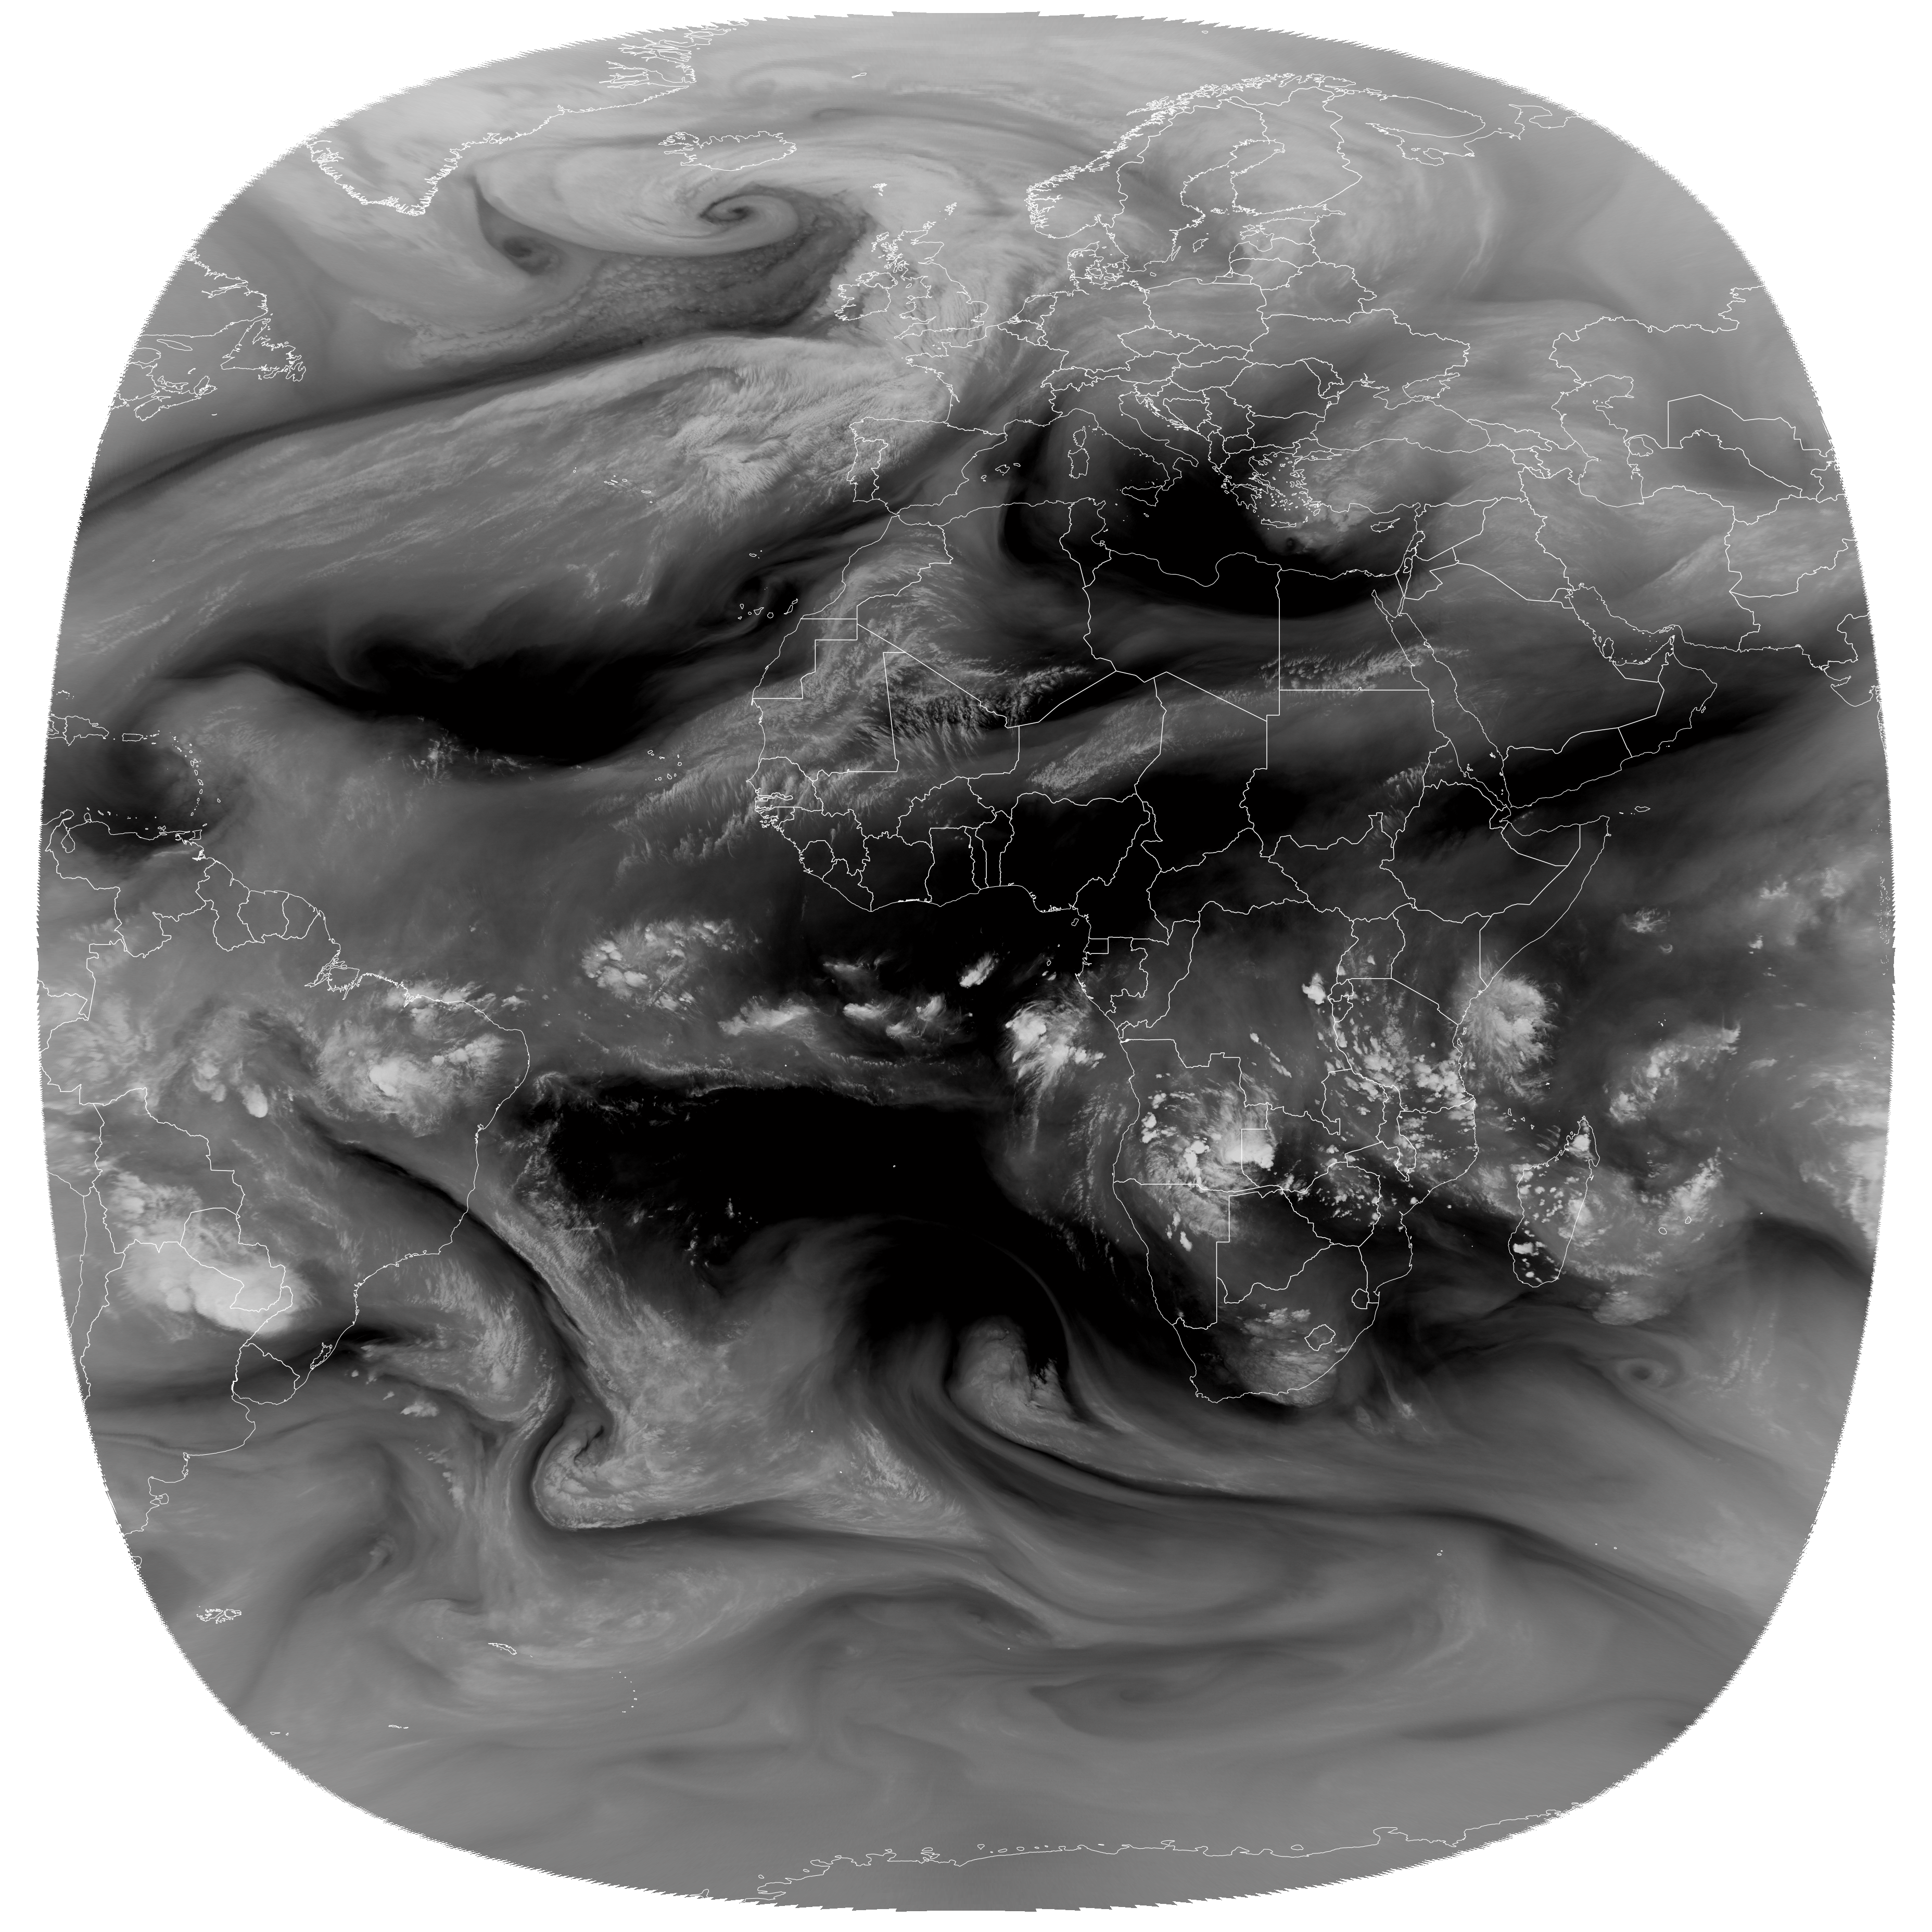
\includegraphics[width=\textwidth]{Chapter2_Theory/images/sat_channels/meteosat-msg_wv062_overlay-ne_10m_coastline_overlay-ne_10m_admin_0_boundary_lines_land.png}
            \caption[Channel WV 6.2]%
            {{\small Channel WV 6.2}}    
            \label{fig:WV_6.2}
        \end{subfigure}
        \hfill
        \begin{subfigure}[b]{0.475\textwidth}  
            \centering 
            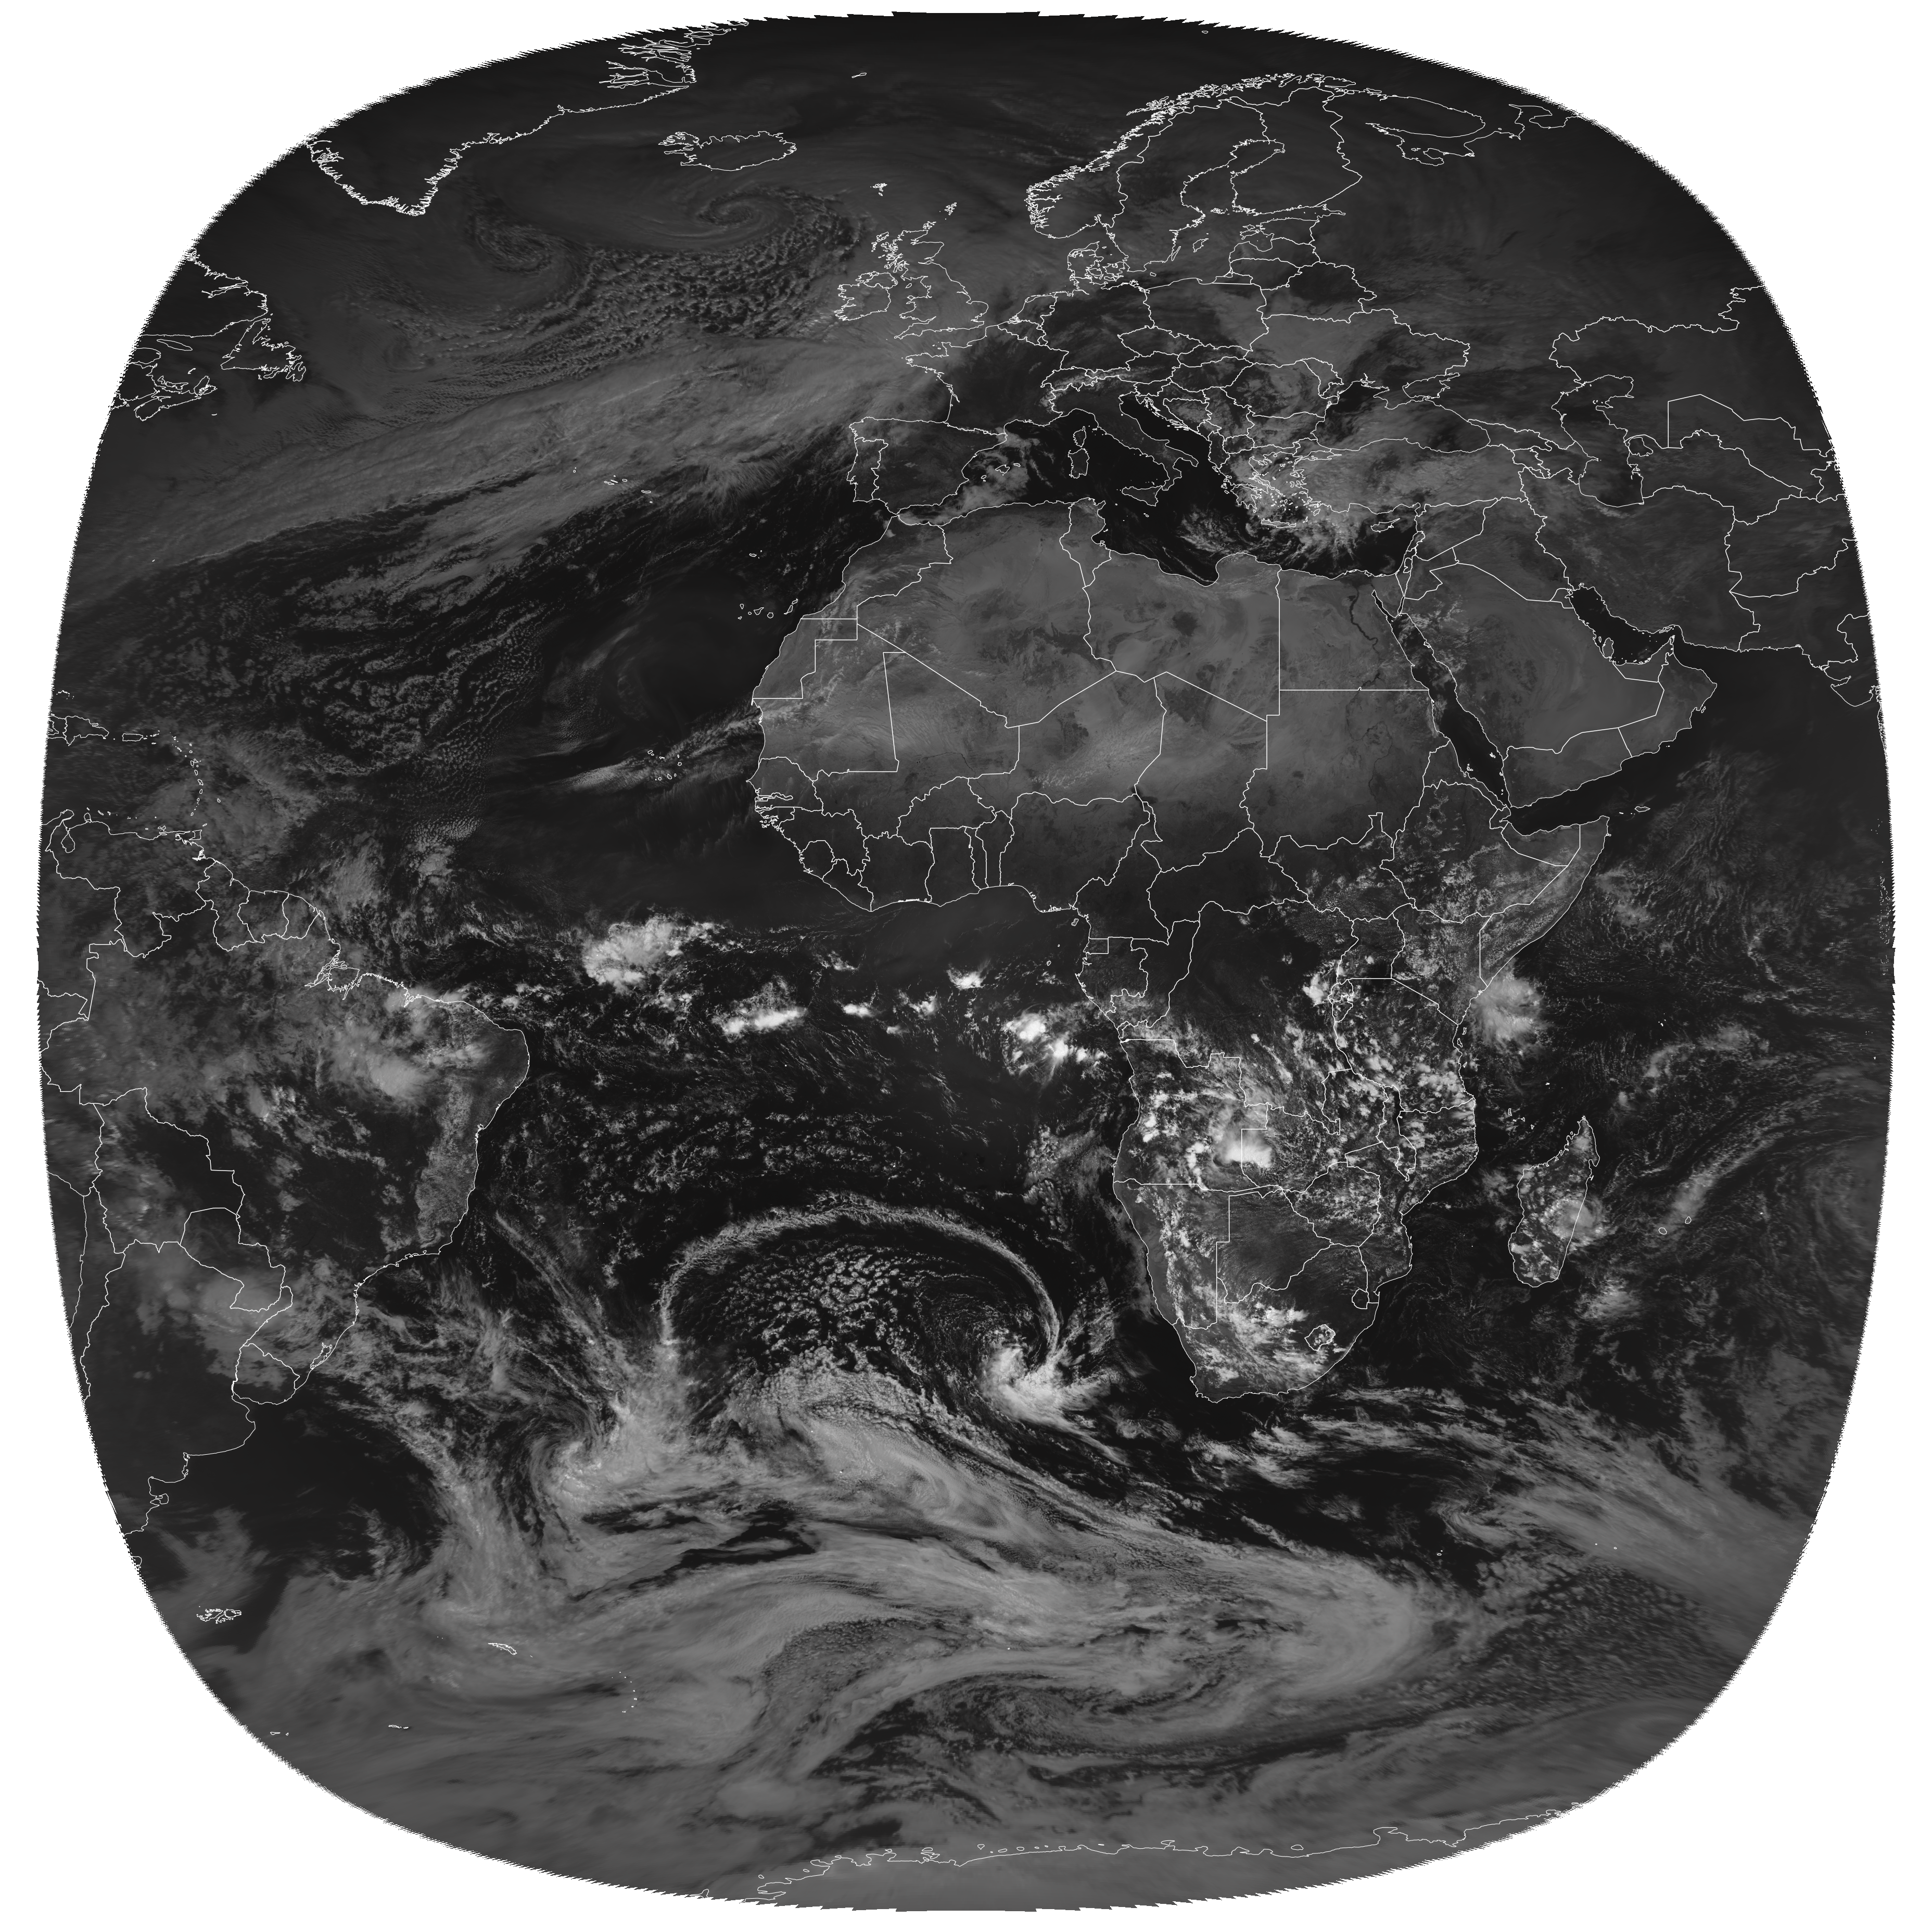
\includegraphics[width=\textwidth]{Chapter2_Theory/images/sat_channels/meteosat-msg_vis006_overlay-ne_10m_coastline_overlay-ne_10m_admin_0_boundary_lines_land.png}
            \caption[]%
            {{\small VIS 0.6}}    
            \label{fig:VIS_0.6}
        \end{subfigure}
        \vskip\baselineskip
        \begin{subfigure}[b]{0.475\textwidth}   
            \centering 
            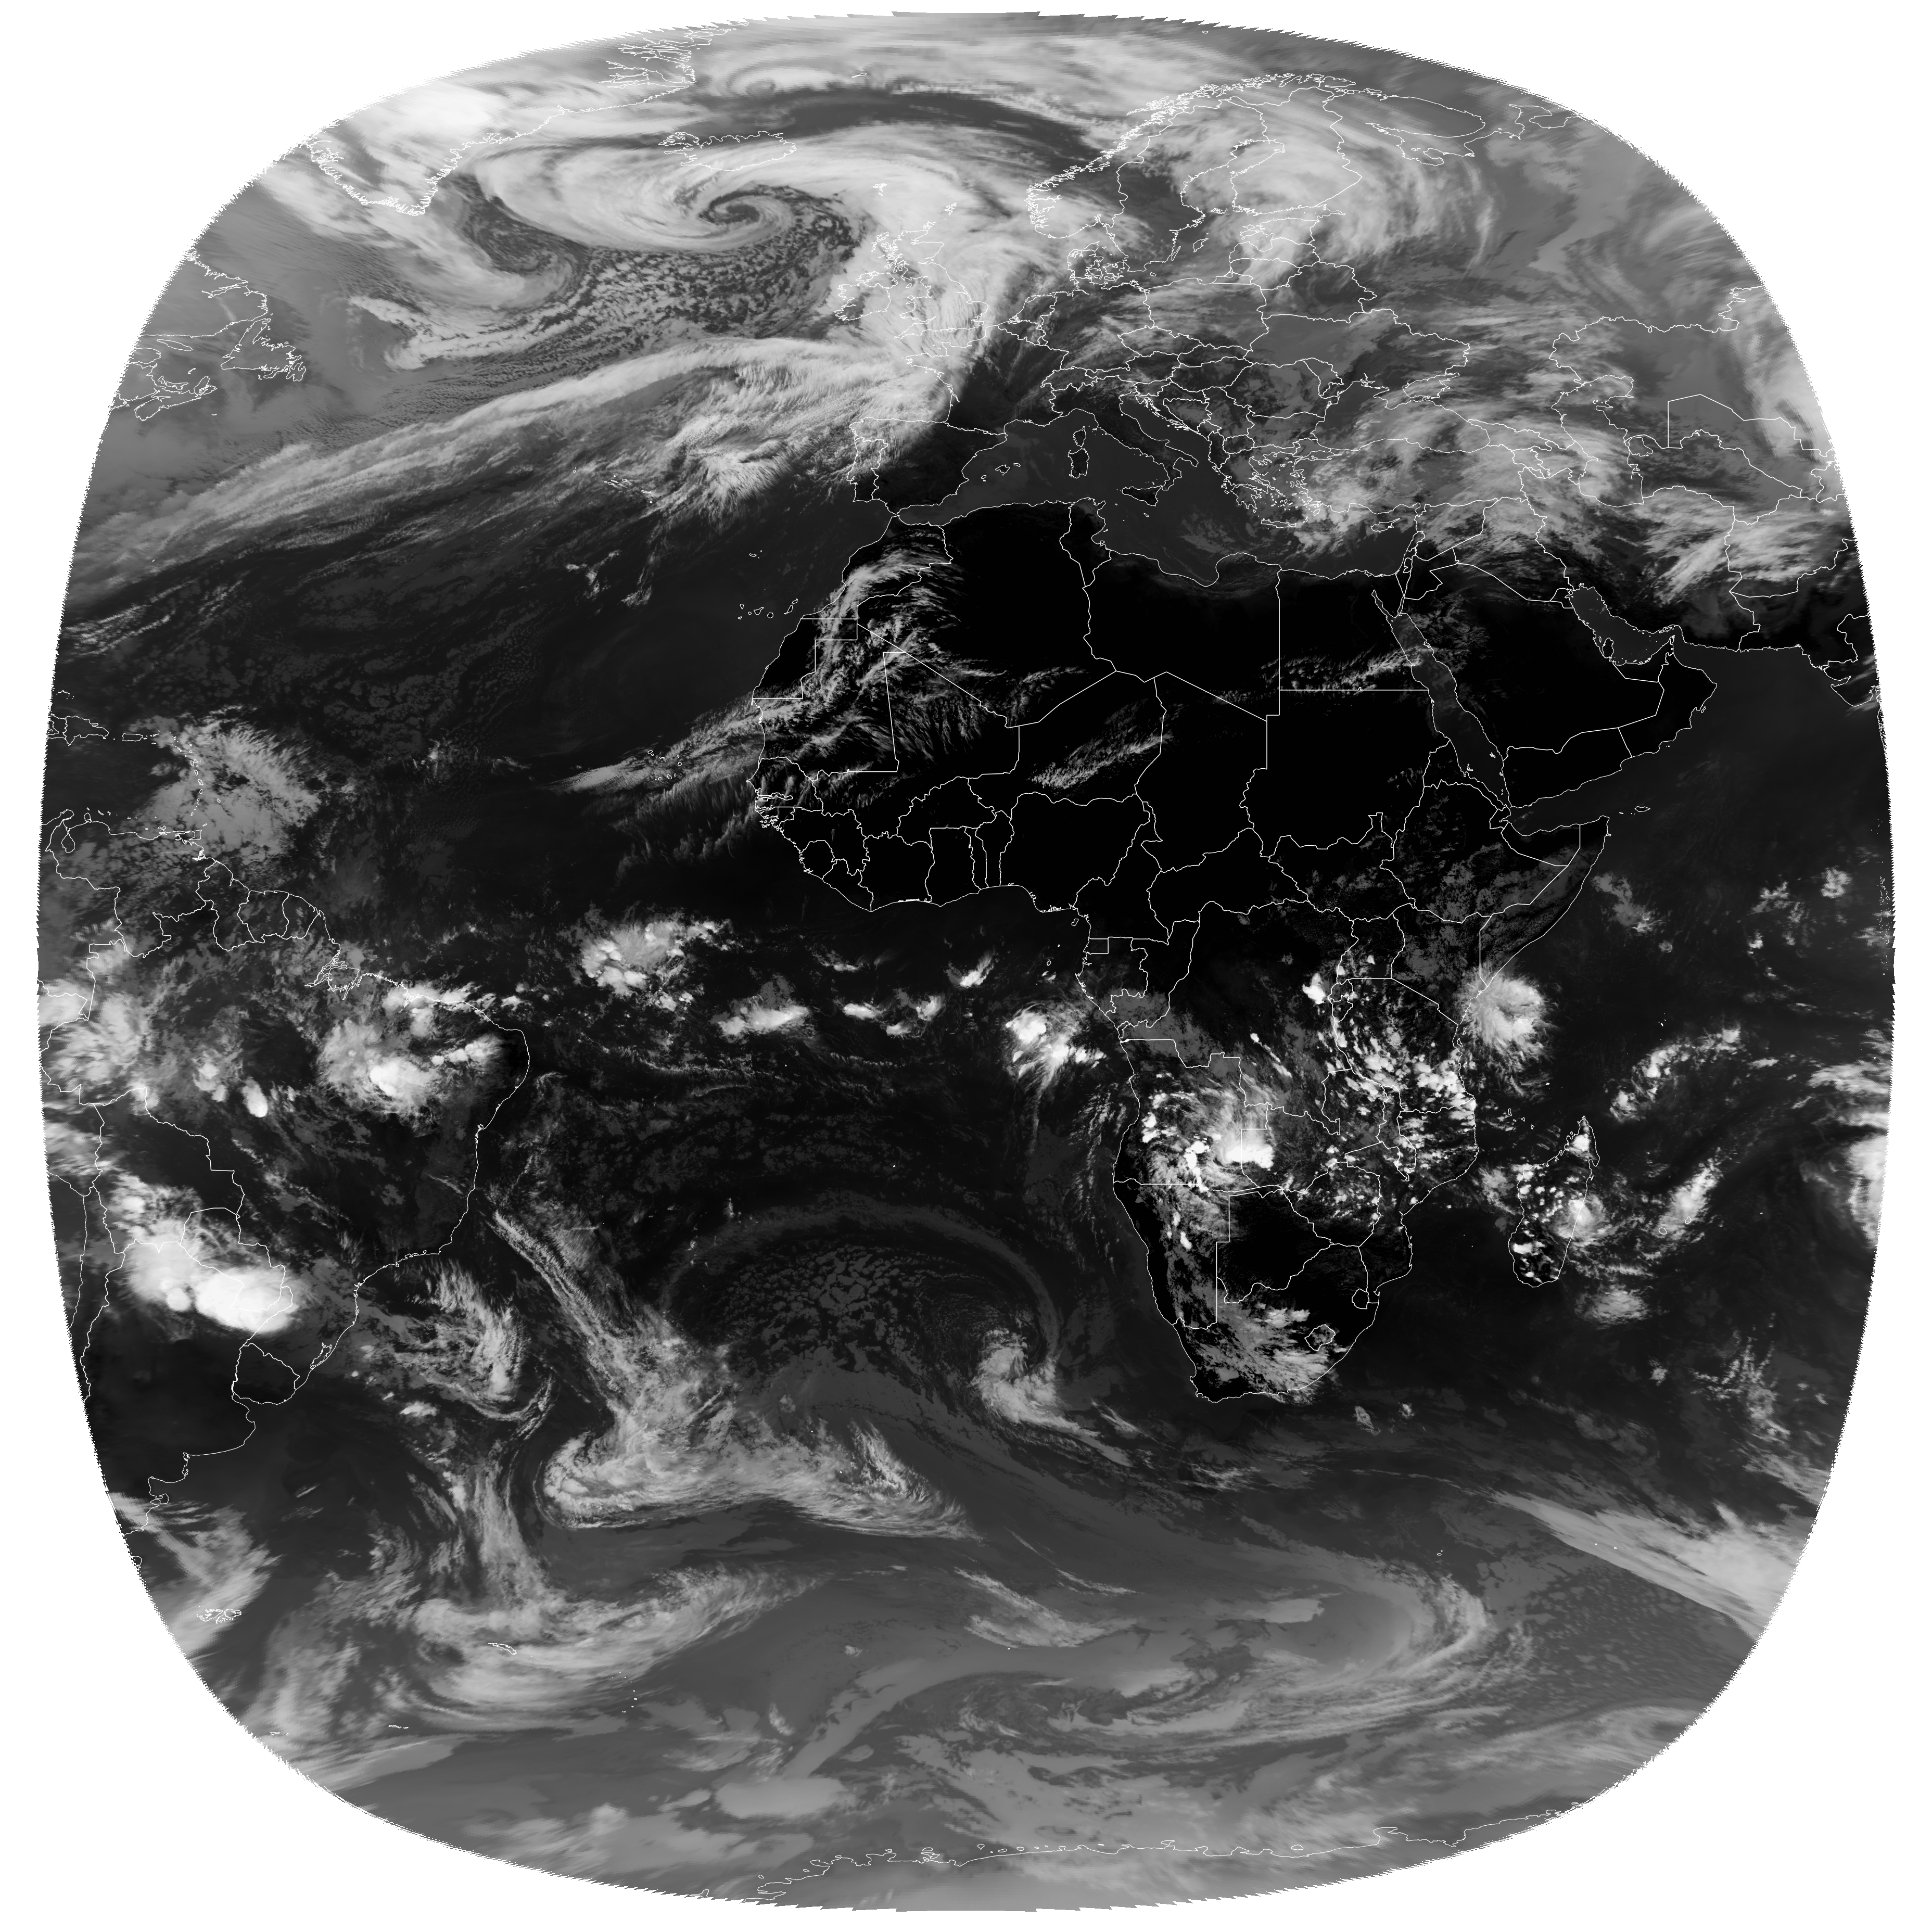
\includegraphics[width=\textwidth]{Chapter2_Theory/images/sat_channels/meteosat-msg_ir108_overlay-ne_10m_coastline_overlay-ne_10m_admin_0_boundary_lines_land.png}
            \caption[something]%
            {{\small IR 10.8}}    
            \label{fig:IR_10.8}
        \end{subfigure}
        \quad
        \begin{subfigure}[b]{0.475\textwidth}   
            \centering 
            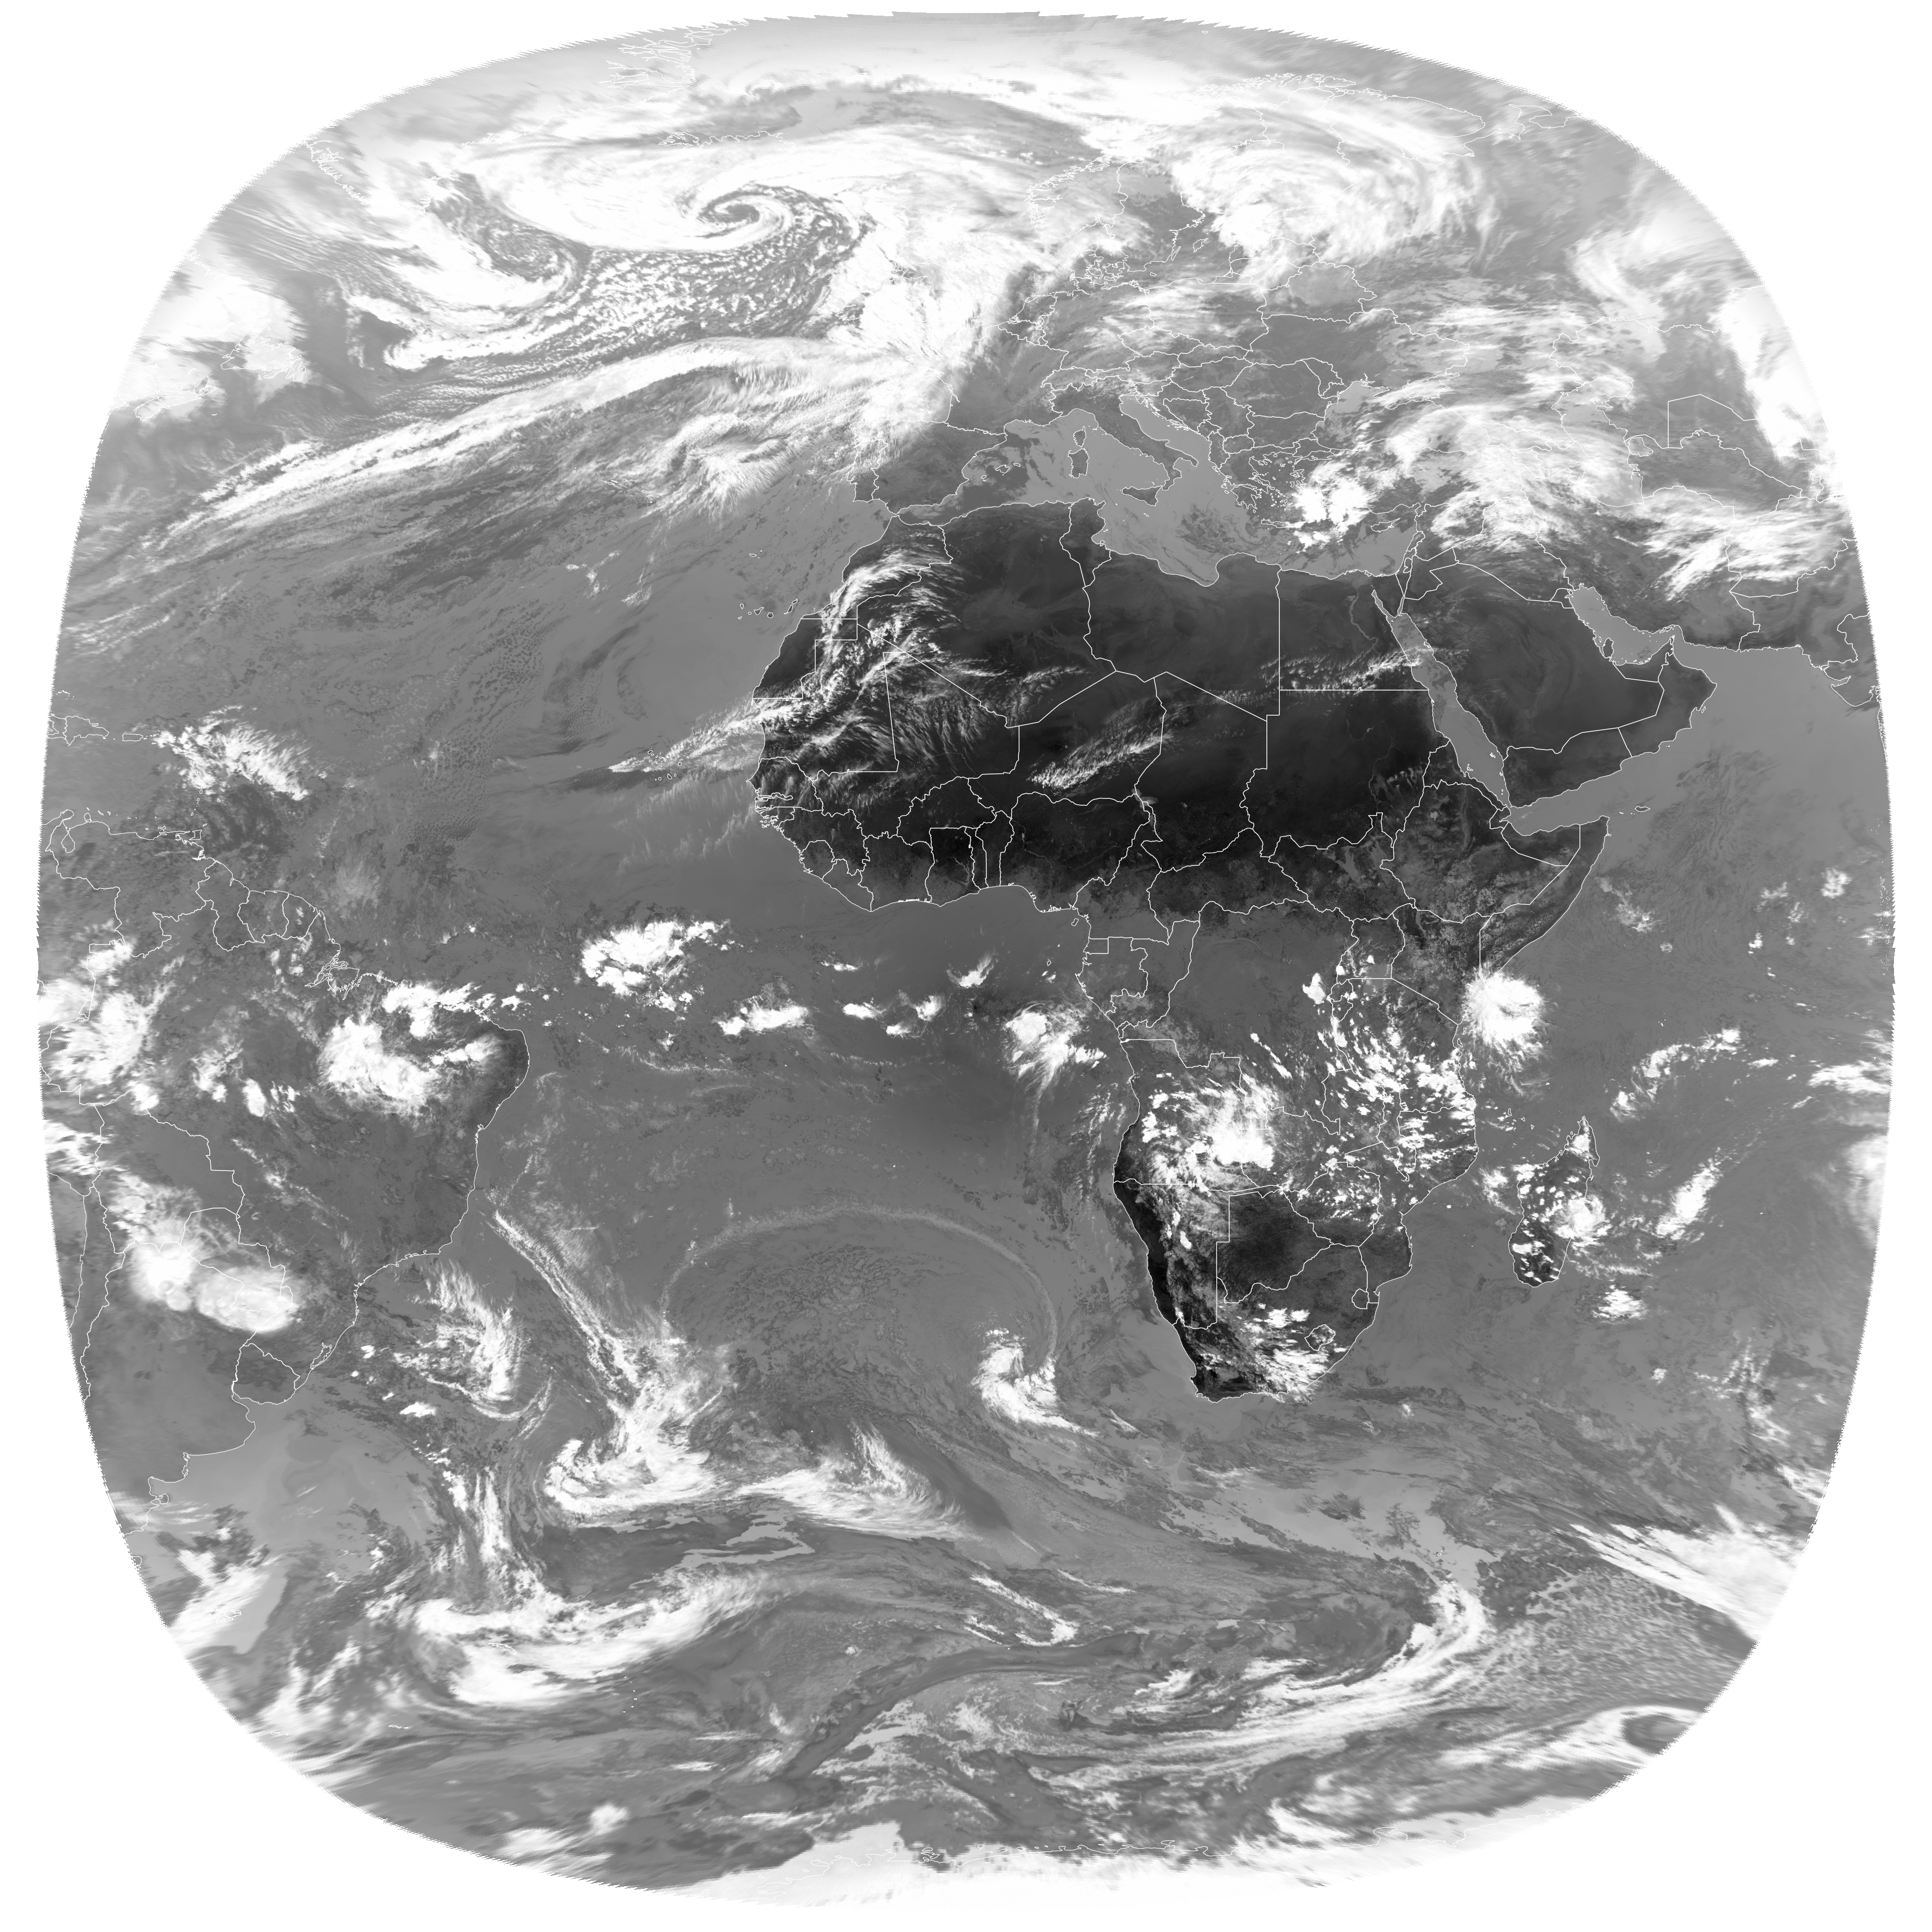
\includegraphics[width=\textwidth]{Chapter2_Theory/images/sat_channels/meteosat-msg_ir039_overlay-ne_10m_coastline_overlay-ne_10m_admin_0_boundary_lines_land.png}
            \caption{{\small IR 3.9}}    
            \label{fig:IR_3.9}
        \end{subfigure}
        \caption{{Spectral bands from SEVIRI. February 15th 2020 at noon. It shows the lowpressure system \textit{Elsa} positioned of the west coast of Iceland. Having a record breaking low of 915hPa (\cite{nrk_lavtrykk}). 
        The images are provided by  \cite{eumetcast_image_gallery}.}
    } 
    \label{fig:SEVIRI_channels}
\end{figure*}

% Info på bildene \textbf{Rectified (level 1.5) Meteosat SEVIRI image data. The data is transmitted as High Rate transmissions in 12 spectral channels. Level 1.5 image data corresponds to the geolocated and radiometrically pre-processed image data, ready for further processing, e.g. the extraction of meteorological products. Any spacecraft specific effects have been removed, and in particular, linearisation and equalisation of the image radiometry has been performed for all SEVIRI channels. The on-board blackbody data has been processed. Both radiometric and geometric quality control information is included. Images are made available with different timeliness according to their latency: quarter-hourly images if latency is more than 3 hours and hourly images if latency is less than 3 hours (for a total of 87 images per day). To enhance the perception for areas which are on the night side of the Earth a different mapping with increased contrast is applied for IR3.9 product. The greyscale mapping is based on the EBBT which allows to map the ranges 200 K to 300 K for the night and 250 K to 330 K for the day.}
% Lastet ned 16.02.2020.
Karlsson et. al. 2015 list the five key properties for remote sensing of clouds using passive imagery. To have a reference figure \ref{fig:SEVIRI_channels} shows examples on how different properties are seen by the satellite. This includes the four spectral bands, WV 6.2, VIS 0.6, IR 3.9 and IR 10.8. In general anything that appears bright have a higher reflectance at the \acrfull{toa} than the surface. Lower radiences are displayed in darker colours and brighter is white. Clouds appear bright in VIS and NIR channels, see \ref{fig:VIS_0.6}. Clouds consisting of liquid droplets reflect strongly in SWIR and MWIR. This is shown in figure \ref{fig:IR_3.9}. The earth surface, including snow and ice, appear dark. This allows for detection of low level clouds at night. Exploiting the fact that clouds are not perfectly emitting black bodies. Cloud are typically colder than the earth surface. Cirrus cloud are optically thin, but can be detected using split window channels (IR10.8 and IR12.0) differences. See figure \ref{fig:IR_10.8}. Figure \ref{fig:WV_6.2} shows detected water vapour. In general broken clouds give rise to scattered pattern or texture in images otherwise homogeneous, ice-free ocean for instance. To summaries the success of a screening is dependant on the illumination, the state of the surface and atmosphere. \textbf{kalsson et al} The number of spectral bands and footprint size (pixel resolution) determine the practical application a particular retrieval can be used for. Differences in swath width determine the frequency at a given position. Viewing angle affect the optical properties of the medium (but also its apparent position). \textit{Parallax} describes the apparent shift in position of a object, when you move the observer along a axis. This is a issue in remote sensing. Positions of satellites are moved and high viewing angles may cause similar issues. Since the position of objects is relevant to the viewing angle. A high viewing angle may introduce problems with parallax of high clouds. This factor is negligible when detecting low clouds (Joro et al). Moving the observer (satellite) changes the apparent position of the measurement. Th

Differences in sensitivity and retrieval algorithms contribute to a large spread in global mean cloud amount among different cloud products. In their assessment of global cloud datasets Studbenau et. al. 2013 compared the global mean cloud cover of six datasets (ISCCP, PATMOS-x, MODIS-ST, MODIS-CE, AIR-LMD and TOVS Path-B). In this process they eliminating MISR and ATSR-GRAPE because of different observation times \textbf{(ref the table in the article)} and two outlier datasets, HIRS-NOAA and POLDER. Their results show that the difference among the six datasets, the difference is of order 0.08. On the contrary, local differences could be up to 0.4. Its worth noting that the satellite data using in this thesis is not included in Schubanaus study, but its illustrates nicely the large differences among other datasets. 

%Cloud-Aerosol Lidar and Infrared Pathfinder Satellite Observations, CALISO is much used in other research because it gives a vertically resolved cloud (3D observations). This additional spatial information is provided on the expense of frequency and uncertainty. \textit{Reason why calipso is ruled out as a candidate. large uncertainty Stubenau} MODIS has low spatial resolution but high temporal resolution, one to two days. National Oceanic and Atmospheric Administration, NOAA \textbf{ something}. Most polar orbiting satellites have a resolution at best daily. \textbf{kilde (shubenau)} \textbf{Does the other one give ferdig produkter av skyfraksjoner og eller er mye lettere og regridde??} The number of channels (higher for other than METEOSAT). The more channels you have the more accurate cloud detection algorihms you can use. Most of the uncertainty in satellite retrivals are attributed to the presence of clouds.  

\textbf{Hugo how much where you thinking of including from other satellites.}

\subsection{METeosat Second Generation, MSG} \label{sec:meteosat}
Prior to the launch of the METeosat researchers discussed the temporal frequency suitable for the observing weather. The METeosat first generation had a temporal resolution of 30min \textbf{kilde}. For the second generation, 15min intervals was chosen to best cope with the short lifetime and rapid deformation of clouds. It was also suggested that a temporal frequency of 1 to 10min is necessary tracking cumulus type clouds. \textbf{kilde stubenau - må være en annen kilde}. This agrees with the table 1.3 in Lohmann et. al. stating the lifetimes of different type clouds. \textbf{kilde Lohmann s. 19} There is a \textit{ring} of geostationary satellites located at equator providing a global covering (not included polar regions). The altitude of satellite determine the forward velocity and is chosen for the geostationary orbit. To achieve this orbit it needs to maintain a height of $\sim 36 000km $. The first Meteosat Second Generation (MSG-1) was lauched 28 August 2002. It became operational 29 January 2004 and got renamed Meteosat-8. The \acrshort{msg} system provides a two satellite system, one operational and one standby. This introduces issues related to the parallax. It becomes evident when comparing simultaneous measurements for the operation and the standby METeosat satellites. \ref{tab:dataset_summary} The operational satellite at a nadir point of $0^o$ latitude. Samples a full disk in cycles of 15min. A full disk is $3712\times 3712$ pixels.
%\textbf{Thoughts:}
%\begin{enumerate}
%    \item Would it be possible to see further north if the altitude where higher? (Wouldn't be geostationary anymore but would you.)
%    \item Må den alltid være på latitude = 0 for å være geostationary? 
%\end{enumerate}
%METeosat is the only geostationary satellite covering the Europe, Africa and India?. Geostationary \textit{ring} of GEO-satellites. 
The \acrfull{msg} was established as a corporation between \acrfull{esa} and \acrfull{eumetsat}. \acrshort{esa} was in charge of developing the prototype of MSG-1. \acrshort{eumetsat} is responsible for maintaining the user requirements, launch procedures, developing ground segments, ensuring over all system consistency and day to day operations.  \acrshort{msg} primary function is to provide a continuous observations of the earths full disk. Near-constant sampling frequency and a geostationary orbit allows for observing weather phenomena occurring on short scales. Since the satellite always is located at $0^o$ the spatial resolution is not constant spatial resolution, unlike the polar orbiting satellites. The resolution becomes coarser with increasing off-nadir viewing angle. \textbf{kilde stubenau} There are efforts invested in extending the MSG dataset with the MFG, in order to make use of the timeseries all the way back to 1980. \textbf{kilde, launched 1977} This is requires new cloud detection algorithms since they only have three common channels and two of them are useful for detecting clouds. \textbf{kilde Stöckli} This could potentially be useful in the future. 

On board the \acrshort{msg} is the \acrfull{seviri} imaging radiometer. Its has  12 spectral channels. The scan is done south to north, east to west. The wavelength of the discrete channels are chosen based on heritage from other sensors. One broadband visible channel, three solar channels (0.6, 0.8 and 1.6 $\mu m$) and 8 thermal infrared channels (3.9, 6.2, 7.3, 8.7, 9.7, 10.8, 12.0 and 13.4 $\mu m$). (Taravat, 2015)  This is of great advantage since much of the community already know how to use the \acrshort{seviri} radiance observations. The channels have been chosen based on their ability to detect clouds, water vapour and ozone. More information about what the different channels detect is available in this paper \textit{An introduction to METeosat second generation (MSG)} published in BAMS 2002 \textbf{kilde Schmetz}. % \ref{tab:dataset_summary}. 
\begin{figure}[h]
    \centering
    \includegraphics[scale=0.11]{Chapter2_Theory/images/MET10_RGBNatColourEnhncd_FullResolution_20191123120000.jpg}    
    \caption{\textit{Coverage with \acrshort{seviri} on MSG.}The view of the earth from \acrshort{msg}. The picture is dated noon on the 11 November 2019. \textbf{Cite EUMETSAT}. By studying the patterns it becomes evident that clouds are influenced by the circulations. The image is "Natural colors enhanced"}
    \label{fig:sat_view}
\end{figure}
%You may calculate the difference of the measurements, e.g. for channels VIS0.6, IR3.9 and IR10.8 between the two satellites. This will give an estimate how large the measurements differ and as a consequence the products (e.g. cloud mask) will be different.\textbf{also personal correspondance.}
The operational cloud detection algorithm is pixel by pixel. Post processing involves re-classifing isolated pixels. There is a lot of effort invested in new detection algorithms including spatial structures. One of the methods that show potential here is deep learning \textbf{List many sources.}

The viewing angle attributes to small differences in detected cloud mask. Explained by parallax. This becomes evident when the standby and operational satellite scan simultaneously. By default the standby satellite is adjusted to fit the position of the operational. By taking the difference some small patterns becomes visible. This is not accounted/adjusted for when using the data. Sometimes both satellites gather data at the same time. Then the standby-satellite grid is rectified to a a grid of the operational one \textbf{(Personal correspondence EUMETSAT staff).} 

\subsection{EUMETSAT Cloud Mask} \label{sec:EUMETSAT_cloud_mask}

The \acrshort{eumetsat} cloud mask, CLM consist of four classes, described in table \ref{tab:classes_clm}.

\begin{table}[]
    \centering
    \begin{tabular}{c|c}
        Class & Description \\ \hline
        0 & Clear sky over ocean \\
        1 & Clear sky over land \\
        2 & Cloudy \\
        3 & No data/ outer space        
    \end{tabular}
    \caption{Description of classes in EUMETSAT Cloud Mask product.}
    \label{tab:classes_clm}
\end{table}

\begin{table}[]
    \centering
    \begin{tabular}{c|c}
        Spectral band & Central wavelength $\left( \mu m  \right)$ \\ \hline
        VIS 0.6 & 0.635 \\
        VIS 0.8 & 0.81 \\
        NIR 1.6 & 1.64 \\
        IR 3.9 & 3.92 \\
        WV 6.2 & 6.25 \\
        WV 7.3 & 7.35 \\ 
        IR 8.7 & 8.7 \\
        IR 9.7 & 9.66 \\
        IR 10.8 & 10.8 \\
        IR 12.0 & 12 \\
        IR 13.4 & 13.4 \\
        HRV & 0.75
    \end{tabular}
    \caption{List of MSG spectral bands and their central wavelength. \textbf{Expand this with a column of what they are useful to detect. Move table to MSG section. } All of these channels are useful when detection clouds except on? Add subplots of images in the different channels. See Schmetz et. al. 2002  Not refered to anywhere yet.}
    \label{tab:msg_spectral_bands}
\end{table}
These classes are derived from almost all channels except HRV and isolated pixels are reclassified \textbf{cite article 10 in Tavarat, 2015}. The cloud mask is distributed in GRIdded Binary or General Regularly-distributed Information in Binary form (GRIB) (no coordinates) and network Common Data Form (NetCDF) (coordinates). The data is available on Earth Observation Portal on EUMETSATS web pages. 

%\begin{figure}[h]
%    \centering
%    \includegraphics[scale = 0.6]{Chapter2_Theory/images/coordinates.png}
%    \caption{Credit, https://tex.stackexchange.com/questions/159445/draw-in-cylindrical-and-spherical-coordinates}
%    \label{fig:coords}
%\end{figure}
%The cloud cover will be referred to as cloud amount, fraction or simply the clouds.
%%%%%%%%%%%%%%%%%%%%%%%%%%%%%%%%%%%%%%%%%%%%%%%%%%%%%%%%%%%%%
\subsection{Maskinlæring}
Present general methods.

\subsubsection{LSTM}
a

\subsection{AR}
b


\section{Practical implications - OUTDATED} \label{sec:practical_implications}
It is necessary to have a understanding of the needs of the end product before conducting large machine learning projects. Answering questions like: What will it be used for and how can it be implemented in useful way?

A major downside of the data driven learning approach is the rigid resolution. A trained model can only be used on similar problems, with the same spatiotemporal resolution. For applications like climate models, output comes in a wide range of different resolutions. Before implementing the finished product in a new model of a different resolution, it would need to be retrained on the resolution of the climate model under development. This process involves both remapping of the dataset and retraining the model at the correct resolution. This is a time consuming process involving finding a new set of hyperparameters suitable for the new resolution. % It essentially means starting over.

Once trained on global climate datasets, machine learning models provide fast results even for complex parameterisation which is what makes them suitable for the application of climate modelling. Most machine learning packages are developed using Python. \acrfull{esm} are implemented in python. Methods for including the trained parameterizations need to be developed.
 
\subsection{Any implications based on the results presented in this chapter.}

\subsubsection{summary}
This thesis aim to devolop and/or explore methods of parameterising cloud cover based on macro-scale variables like humidity, surface temperature and pressure. Regressing historical observations against macro physical properties which affect clouds. Moving away from the subgrid scale processes. Wish to answar weather there be enough information in humidity, temperature and surface pressure to predict clouds in a time and space.



% Kommentarer fra Hugo om skriving : Teoridelem om satelitter hva er nevn flere og deres oppløsning og hva er fordelen og ulemepen med dem. 
%  Legg inn helt generelle ting i teoretical background åså diskuter selve datasettet i metoden.

% Ignorer artifakten men kommenter i resultatene, keep in mind the artifact is present. 
% Fixed input length, normally one would add 0 if it not present. We need to find a value to add. 
% Scaling is smart due to numerical error not necessarily a requirement for the statistical models. 
% Missing values can be dealt with in two ways. 
% 1) Calculate the average ()
% 2) Predict the missing values - as always this might lead to a unnatural smoothness. 
% 3) 